
\begin{columns}
\begin{column}{.5\linewidth}
\begin{center}
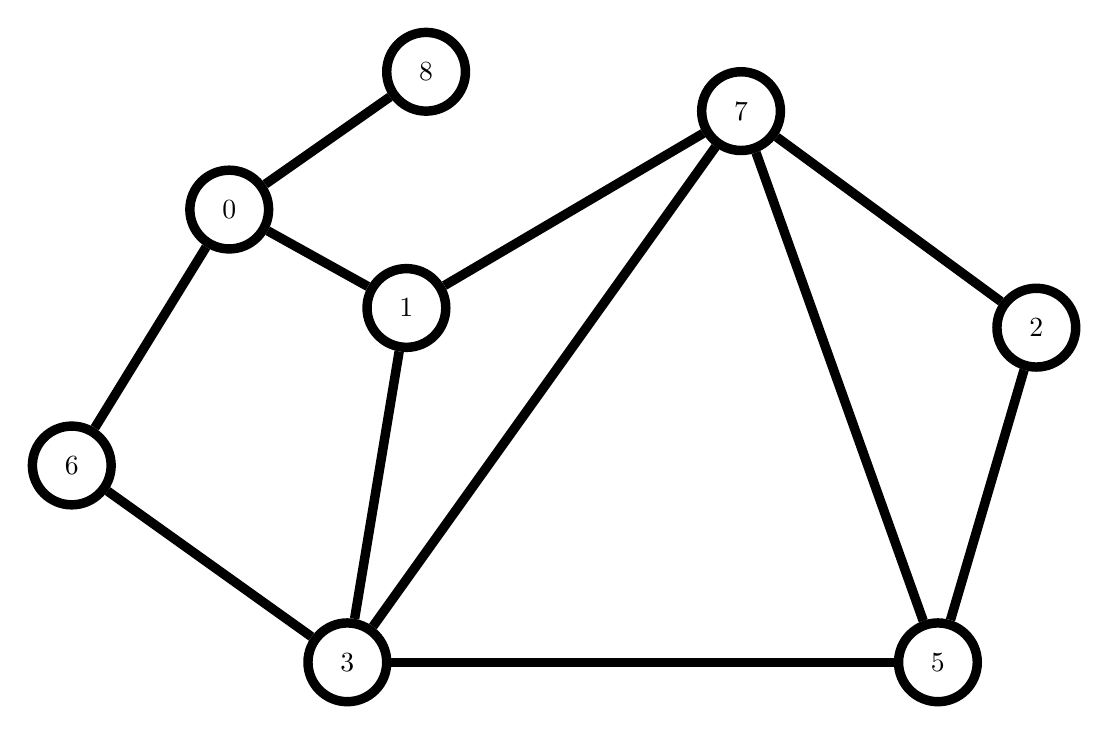
\begin{tikzpicture}[scale=2.5]
\tikzstyle{mythick}=[line width=.12cm];
\tikzstyle{gn}=[draw=black,circle,thick,inner sep=7pt,minimum size=1cm,mythick]
\tikzstyle{ed}=[draw=black,mythick]
\node [gn] (a) at (0,0) {$3$};
\node [gn] (b) at (3,0) {$5$};
\node [gn] (c) at (2,2.8) {$7$};
\node [gn] (d) at (3.5,1.7) {$2$};
\node [gn] (e) at (-1.4, 1) {$6$};
\node [gn] (f) at (.4,3.0) {$8$};
\node [gn] (g) at (.3,1.8) {$1$};
\node [gn] (h) at (-.6,2.3) {$0$};
\draw [ed] (a) -- (b);
\draw [ed] (c) -- (d);
\draw [ed] (a) -- (e);
\draw [ed] (d) -- (b);
\draw [ed] (a) -- (c);
\draw [ed] (b) -- (c);
\draw [ed] (a) -- (g);
\draw [ed] (g) -- (c);
\draw [ed] (g) -- (h);
\draw [ed] (e) -- (h);
\draw [ed] (f) -- (h);
\end{tikzpicture}

Input
\end{center}
\end{column}
\begin{column}{.5\linewidth}
\begin{center}
\begin{tikzpicture}[scale=2.5]
\tikzstyle{mythick}=[line width=.12cm];
\tikzstyle{gn}=[draw=black,circle,thick,inner sep=7pt,minimum size=1cm,mythick]
\tikzstyle{ed}=[draw=black,mythick]
\tikzstyle{selection}=[double=blue!20,double distance=60pt,line width=.2cm,draw=blue!50,line cap=round,line join=round];
\node [gn] (a) at (0,0) {$3$};
\node [gn] (b) at (3,0) {$5$};
\node [gn] (c) at (2,2.8) {$7$};
\node [gn] (d) at (3.5,1.7) {$2$};
\node [gn] (e) at (-1.4, 1) {$6$};
\node [gn] (f) at (.4,3.0) {$8$};
\node [gn] (g) at (.3,1.8) {$1$};
\node [gn] (h) at (-.6,2.3) {$0$};
\draw [ed] (a) -- (b);
\draw [ed] (c) -- (d);
\draw [ed] (a) -- (e);
\draw [ed] (d) -- (b);
\draw [ed] (a) -- (c);
\draw [ed] (b) -- (c);
\draw [ed] (a) -- (g);
\draw [ed] (g) -- (c);
\draw [ed] (g) -- (h);
\draw [ed] (e) -- (h);
\draw [ed] (f) -- (h);
\begin{scope}[on background layer]
\draw [selection] (0,0) -- (3,0) -- (2,2.8);
\end{scope}
\end{tikzpicture}

Output
\end{center}
\end{column}
\end{columns}

\vspace{1.2cm}

We solve \textbf{approximate} versions of the projection problem via reductions to the \textbf{prize-collecting Steiner tree problem} (PCST).\\[1.5cm]

\textbf{Objective of PCST:} Given a graph with edge costs $c$ and node prizes $\pi$, find a subtree $T$ minimizing $c(T) + \pi(\overline{T})$.

\vspace{.7cm}

\begin{columns}
\begin{column}{.5\linewidth}
\begin{center}
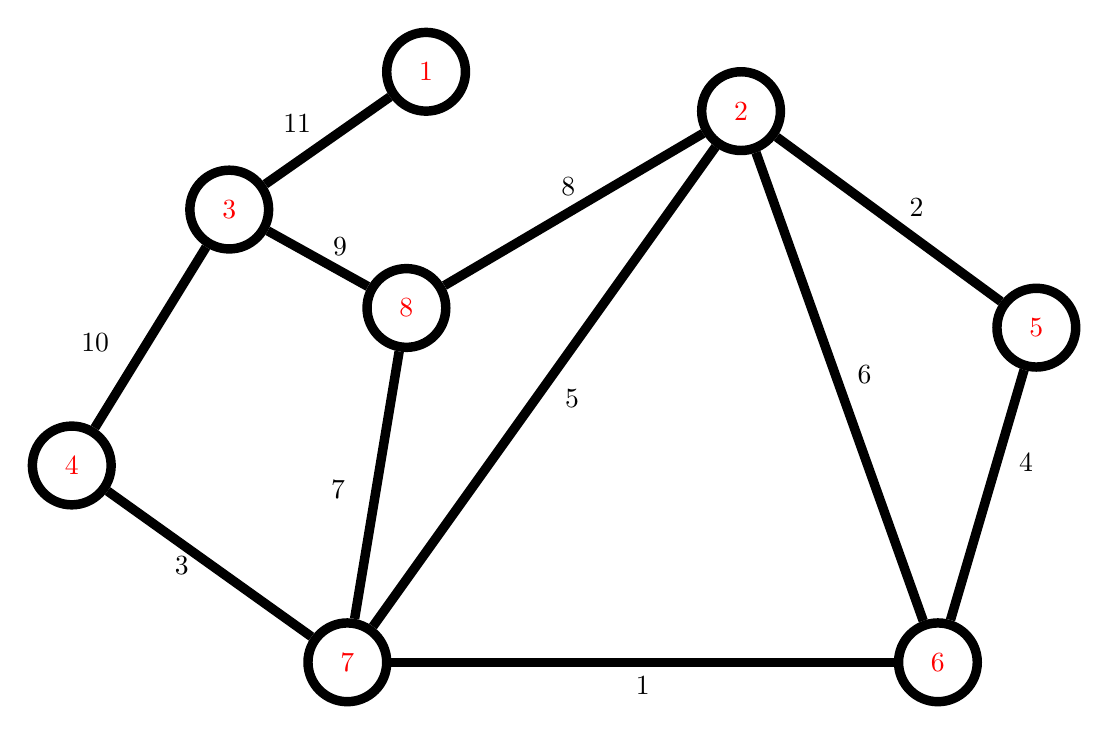
\begin{tikzpicture}[scale=2.5]
\tikzstyle{mythick}=[line width=.12cm];
\tikzstyle{gn}=[draw=black,circle,thick,inner sep=7pt,minimum size=1cm,mythick,text=red]
\tikzstyle{ed}=[draw=black,mythick]
\tikzstyle{selection}=[double=blue!20,double distance=60pt,line width=.2cm,draw=blue!50,line cap=round,line join=round];
\node [gn] (a) at (0,0) {7};
\node [gn] (b) at (3,0) {6};
\node [gn] (c) at (2,2.8) {2};
\node [gn] (d) at (3.5,1.7) {5};
\node [gn] (e) at (-1.4, 1) {4};
\node [gn] (f) at (.4,3.0) {1};
\node [gn] (g) at (.3,1.8) {8};
\node [gn] (h) at (-.6,2.3) {3};
\draw [ed] (a) -- (b) node [below,midway] {1};
\draw [ed] (c) -- (d) node [above,midway,xshift=10pt,yshift=-4pt] {2};
\draw [ed] (a) -- (e) node [below=-7.5pt,midway,xshift=-10pt] {3};
\draw [ed] (d) -- (b) node [below=-20pt,midway,xshift=14pt] {4};
\draw [ed] (a) -- (c) node [below=-4pt,midway,xshift=10pt] {5};
\draw [ed] (b) -- (c) node [above=-4pt,midway,xshift=9pt] {6};
\draw [ed] (a) -- (g) node [above=-10pt,midway,xshift=-14pt] {7};
\draw [ed] (g) -- (c) node [above,midway,xshift=-2pt] {8};
\draw [ed] (g) -- (h) node [above=-4pt,midway,xshift=8pt] {9};
\draw [ed] (e) -- (h) node [above=-10pt,midway,xshift=-20pt] {10};
\draw [ed] (f) -- (h) node [above=-2pt,midway,xshift=-11pt] {11};
\end{tikzpicture}

Input
\end{center}
\end{column}
\begin{column}{.5\linewidth}
\begin{center}
\begin{tikzpicture}[scale=2.5]
\tikzstyle{mythick}=[line width=.12cm];
\tikzstyle{gn}=[draw=black,circle,thick,inner sep=7pt,minimum size=1cm,mythick,text=red]
\tikzstyle{ed}=[draw=black,mythick]
\tikzstyle{selection}=[double=blue!20,double distance=60pt,line width=.2cm,draw=blue!50,line cap=round,line join=round];
\node [gn] (a) at (0,0) {7};
\node [gn] (b) at (3,0) {6};
\node [gn] (c) at (2,2.8) {2};
\node [gn] (d) at (3.5,1.7) {5};
\node [gn] (e) at (-1.4, 1) {4};
\node [gn] (f) at (.4,3.0) {1};
\node [gn] (g) at (.3,1.8) {8};
\node [gn] (h) at (-.6,2.3) {3};
\draw [ed] (a) -- (b) node [below,midway] {1};
\draw [ed] (c) -- (d) node [above,midway,xshift=10pt,yshift=-4pt] {2};
\draw [ed] (a) -- (e) node [below=-7.5pt,midway,xshift=-10pt] {3};
\draw [ed] (d) -- (b) node [below=-20pt,midway,xshift=14pt] {4};
\draw [ed] (a) -- (c) node [below=-4pt,midway,xshift=10pt] {5};
\draw [ed] (b) -- (c) node [above=-4pt,midway,xshift=9pt] {6};
\draw [ed] (a) -- (g) node [above=-10pt,midway,xshift=-14pt] {7};
\draw [ed] (g) -- (c) node [above,midway,xshift=-2pt] {8};
\draw [ed] (g) -- (h) node [above=-4pt,midway,xshift=8pt] {9};
\draw [ed] (e) -- (h) node [above=-10pt,midway,xshift=-20pt] {10};
\draw [ed] (f) -- (h) node [above=-2pt,midway,xshift=-11pt] {11};
\begin{scope}[on background layer]
\draw [selection] (3.5,1.7) -- (3,0) -- (0,0) -- (-1.4,1) -- (0,0) -- (.3,1.8);
\end{scope}
\end{tikzpicture}

Output
\end{center}
\end{column}
\end{columns}

\vspace{1.5cm}

$\rightarrow$ \textbf{Nearly-linear} time approximate projections.
